%%%%%%%%%%%%% Doing my own template
%%%%%%%%%%%%% Following the specifications of
% http://bu.univ-amu.libguides.com/c.php?g=511743&p=4025195
%%%%%%%%%%%%% Sober amu thesis template

% LAYOUT %%%%%%%%%%%%%%%%%%%%%%%%%%%%%%%%%%%%%%%%%%%%
%%% Using the report class
\documentclass[12pt, 			% Recommended
               twoside,         % SHOULD BE
               %singlespacing
			  ]{report}

%%% Margins
\usepackage[a4paper,
			%width=150mm,
			top=30mm,
			bottom=30mm,
            right=30mm,
            left=30mm,
            % Offset to bind pages
            bindingoffset=6mm,  
            % To make room for the header
            headheight=20mm,    
           ]{geometry}

% Line spacing - 1 is normal, 1.3 is onehalf and 1.6 is double spacing
\linespread{1}

%%% Change titles & stuff
\makeatletter
\renewcommand{\@chapapp}{Section}
\makeatother
\renewcommand{\abstractname}{Résumé}
\renewcommand{\contentsname}{Summary}
\renewcommand{\appendixname}{Table des annexes}

%%%%%%%%%%%%%%%%%%%%%%%%%%%%%%%%%%%%%%%%%%%%%%%%%%%%%

% Miscellaneous packages %%%%%%%%%%%%%%%%%%%%%%%%%%%%

%%% Really basic packages here to handle languages
\usepackage[english]{babel}
\usepackage[utf8]{inputenc}
\usepackage[T1]{fontenc}
% The font
\usepackage{concmath}
% Highlight stuff for revisions + colors and units
\usepackage{color}
\usepackage{enumitem}
\usepackage[x11names]{xcolor}
\usepackage{graphicx}

\usepackage{algorithm}
\usepackage{algorithmic}
\usepackage{amsmath,amssymb, bm}
\usepackage[squaren, Gray, cdot]{SIunits}

% Where your pictures are
\graphicspath{ {pics/} }

%%% Header & Footer
\usepackage{fancyhdr}
\pagestyle{fancy}
\fancyhead{}
\fancyhead[RO,LE]{\rightmark}
\fancyfoot{}
\fancyfoot[LE,RO]{\thepage}
\fancyfoot[CE,CO]{\leftmark}
\fancyfoot[RE,LO]{Thomas Marquet}
\renewcommand{\headrulewidth}{0.4pt}
\renewcommand{\footrulewidth}{0.4pt}

% Some symbols
\usepackage{textcomp}

% To include pdfs, like articles, directly
\usepackage{pdfpages}            

% For figures
\usepackage{caption}
\usepackage{subcaption}

% For text boxes spanning multiple pages
% And to add a color to it
\usepackage{framed}
% Access the different colors here
% http://mirrors.standaloneinstaller.com/ctan/macros/latex/contrib/xcolor/xcolor.pdf page 40
\colorlet{shadecolor}{LightSteelBlue1}
\colorlet{framecolor}{Blue4}

% New environment for shaded frames
\newenvironment{frshaded}{%
\def\FrameCommand{
\fboxrule=\FrameRule
\fboxsep=\FrameSep
\fcolorbox{framecolor}{shadecolor}
}%
\MakeFramed {\FrameRestore}}%
{\endMakeFramed}
% Use like this
%\begin{frshaded}
%\end{frshaded}

% To make todo notes, exemple in the intro
\usepackage[textwidth=3cm]{todonotes}

% For appendices
\usepackage[toc,page]{appendix}
% And change the names
\renewcommand{\appendixname}{Annexe}
\renewcommand{\appendixtocname}{Annexes}
\renewcommand{\appendixpagename}{Annexes}

% Line breaks in text
% Warning: should find something better for urls >.<
\sloppy

% Add quotes
\usepackage{dirtytalk}

% Fancy tables
\usepackage{multirow}

% Urls
\usepackage{url}

% for pdf docs to read on computers
% use this when compiling the pdf version (to send by mail)
% comment it when you want to print it
\usepackage{hyperref}

% Package only for the template

%%%%%%%%%%%%%%%%%%%%%%%%%%%%%%%%%%%%%%%%%%%%%%%%%%%%%

% Glossary %%%%%%%%%%%%%%%%%%%%%%%%%%%%%%%%%%%%%%

% if you need a glossary
% \usepackage{glossaries}         
% \makeglossaries

% \newglossaryentry{ABF}{name=ABF, description={Adaptive Biasing Force}}

% Use \newglossaryentry{utc}{name=UTC, description={Coordinated Universal Time}} to add a glossary entry within the document
% Use gls{utc} to use that entry somewhere

%%%%%%%%%%%%%%%%%%%%%%%%%%%%%%%%%%%%%%%%%%%%%%%%%%%%%

% Bibliography %%%%%%%%%%%%%%%%%%%%%%%%%%%%%%%%%%%%%%

% Required to generate language-dependent quotes in the bibliography
\usepackage[autostyle=true]{csquotes}

% Use biber - way better than bibtex
\usepackage[backend=biber,
% 			citestyle=numeric-comp,
%             bibstyle=numeric,
            citestyle=authoryear,
            bibstyle=authoryear,
            %dashed=false,
            sorting=nyt,
            natbib=true,
            doi=true,
            url=false,
            isbn=false,
            eprint=false,
            giveninits=true,
            uniquename=init,
            maxcitenames=1, 
            minbibnames=6, 
            maxbibnames=6
            ]{biblatex}

% The filename of the bibliography
\addbibresource{all.bib}

% Start with roman numbers until the introduction
\pagenumbering{roman}

% handle the abbverviations ?
% Basic abbreviation page here, you can play around with the two "5cm"
% To increase or decrease the spacing between the abbreviation and the words
\usepackage{calc}
\makeatletter
\newcommand{\tocfill}{\cleaders\hbox{$\m@th \mkern\@dotsep mu . \mkern\@dotsep mu$}\hfill}
\makeatother
\newcommand{\abbrlabel}[1]{\makebox[5cm][l]{\textbf{#1}\ \tocfill}}
\newenvironment{abbreviations}{\begin{list}{}{\renewcommand{\makelabel}{\abbrlabel}%
        \setlength{\labelwidth}{5cm}\setlength{\leftmargin}{\labelwidth+\labelsep}%
                                              \setlength{\itemsep}{0pt}}}{\end{list}}
                                              
% crossed text, if you need it
\usepackage[normalem]{ulem}

%%%%%%%%%%%%%%%%%%%%%%%%%%%%%%%%%%%%%%%%%%%%%%%%%%%%%

\begin{document}

%% Title page

\begin{titlepage}
\newcommand{\HRule}{\rule{\linewidth}{0.5mm}} % Defines a new command for the horizontal lines, change thickness here

\center % Center everything on the page
 
%----------------------------------------------------------------------------------------
%	HEADING SECTIONS
%----------------------------------------------------------------------------------------


\includegraphics[width=0.6\textwidth]{csm_AAU_neu_60b57104bf.jpg}

%----------------------------------------------------------------------------------------
%	TITLE SECTION
%----------------------------------------------------------------------------------------

\HRule \\[0.8cm]
{ \huge \bfseries Deep learning for speech commands recognition}\\[0.4cm] % Title of your document
\HRule \\[1.5cm]

\centering
\begin{minipage}{0.4\textwidth}
\begin{flushleft} \large
\emph{Author:}\\
Thomas \textsc{MARQUET} % Your name
\end{flushleft}
\end{minipage}
~
\begin{minipage}{0.4\textwidth}
\begin{flushright} \large
\emph{Supervisor:} \\
Olivier
 \textsc{MARCEAU} % Supervisor's Name
\end{flushright}
\end{minipage}\\[2cm]
\end{titlepage}




\tableofcontents

% \listoffigures

% \listoftables

% MAIN TEXT %%%%%%%%%%%%%%%%%%%%%%%%%%%%%%%%%%%%%%%%%


% normal numbering from here
\pagenumbering{arabic}

%%%% Each chapter is in a different file
%% In the [], how the chapter will be called in the table of contents
%% In the {}, the name of the chapter in the text
%% The chaptermark is the name of the chapter in the footer
%%% You want a small enough chaptermark or it will overflow to the sides
\chapter[Learning Task]{Learning Task}
\chaptermark{Learning Task}
\section{Introduction}
From our devices listening to you and waiting for you to call their names, to removing the language barrier between humans using automated translation, speech recognition is definitively one of the most growing technology. Being able to speak to a computer using the most natural communication vector of them all, will enhance many daily life applications. Many of us lives permanently with at least one computer more powerful than everything that we could think of 20 years ago, and this computer has access to almost infinite calculation power through the cloud with a low latency. Therefore the use of neural networks to enable robust human/computer communication through voice became possible on large scale and outclassed classical techniques.

\section{Task description}

This work is an introduction to speech recognition. We use a public dataset brought by Google called "Google speech commands v1". The task is the classification of 20 differents small words which could be commonly used to give commands to a computer. We'll compare the results of differents type and size of neural networks which are known to fit such tasks.

\vspace{5mm}

The words that we want to learn are the following : "yes" ,  "no" , "stop" , "go" , "down" , "up" , "left" , "right" , "on" , "off" , "zero" , "one" , "two" , "three" , "four", "five" , "six" , "seven" , "eight" , "nine".

\vspace{5mm}

We also want to recognize when there is an other word than those 20. To do so we'll use 10 additionnals words that will be labeled under "unknown". Those words are  :  "marvin", "sheila" , "tree" , "wow" , "bed" , "bird", "dog" , "cat" , "happy" , "house". 

\vspace{5mm}

Finally, we also want to recognize when there is no word spoken. We'll add a silence label.


\chapter[Data analysis]{Data analysis}
\chaptermark{Data analysis}
\section{Data's distribution}

The dataset is composed of 70k .wav files which are already split ( training set : 58252 , validation set : 6137 , test set : 6231 ). Those files are regrouped in 30 differents words that can be learned. You can also find 6 extra files of differents length which are just common noises.


\begin{figure}[!h]
    \centering
    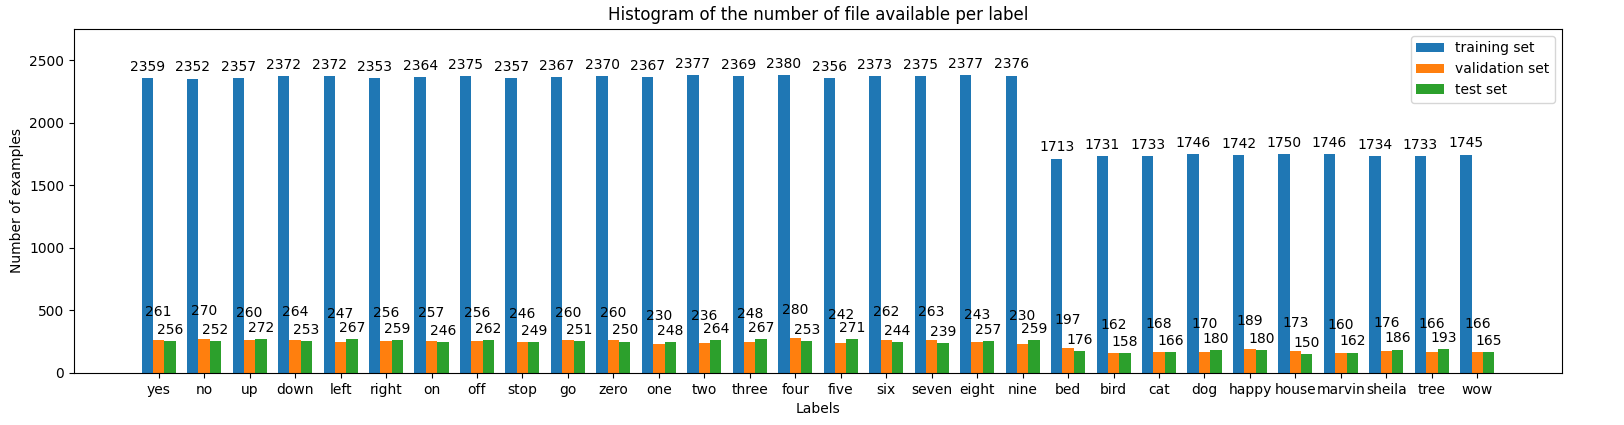
\includegraphics[width=1\textwidth]{chapters/pictures/histo_all.PNG}
    \caption{Files distributions}
    \label{fig:init_dist}
\end{figure}


Each file is supposed to contain a one second clip recorded at a rate of 16kHz. Therefore we should expect 16000 points once the file is loaded, but plenty of them are actually not one second long. This will bring problems later on since we need the inputs to be always the same length. We can either expend those data to get the same length as the others ( zero-padding, averaging, ...), we can cut the silences out of every file and take only the voices, or we can simply ignore them.



\begin{figure}[!h]
    \centering
    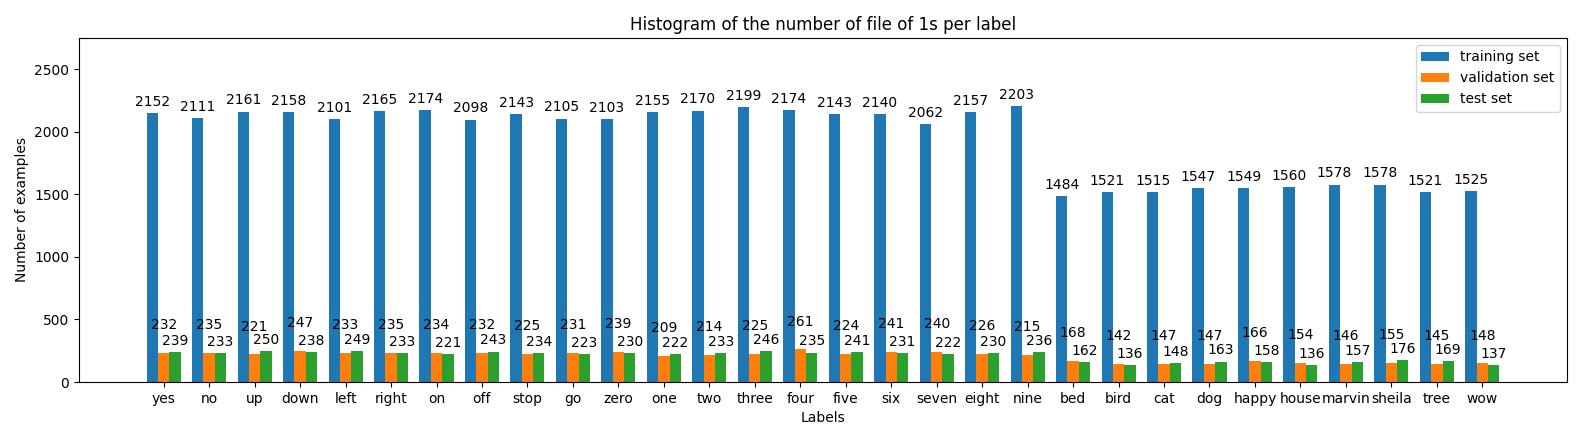
\includegraphics[width=1\textwidth]{chapters/pictures/histo_all_1s.PNG}
    \caption{Files of 1s distributions}
    \label{fig:init_dist_1s}
\end{figure}

\newpage

\section{Raw data : Does it makes sense to use them ?}

Even if audio raw files can be fed to a network and lead to a success while building really deep CNN structures, we're looking for lightweight networks and we have to highlights features to make the learning easier. Fortunately our data is relatively clean of any noise, and therefore we still can detect some patterns from the raw data. 

\begin{figure}[!h]
    \centering
    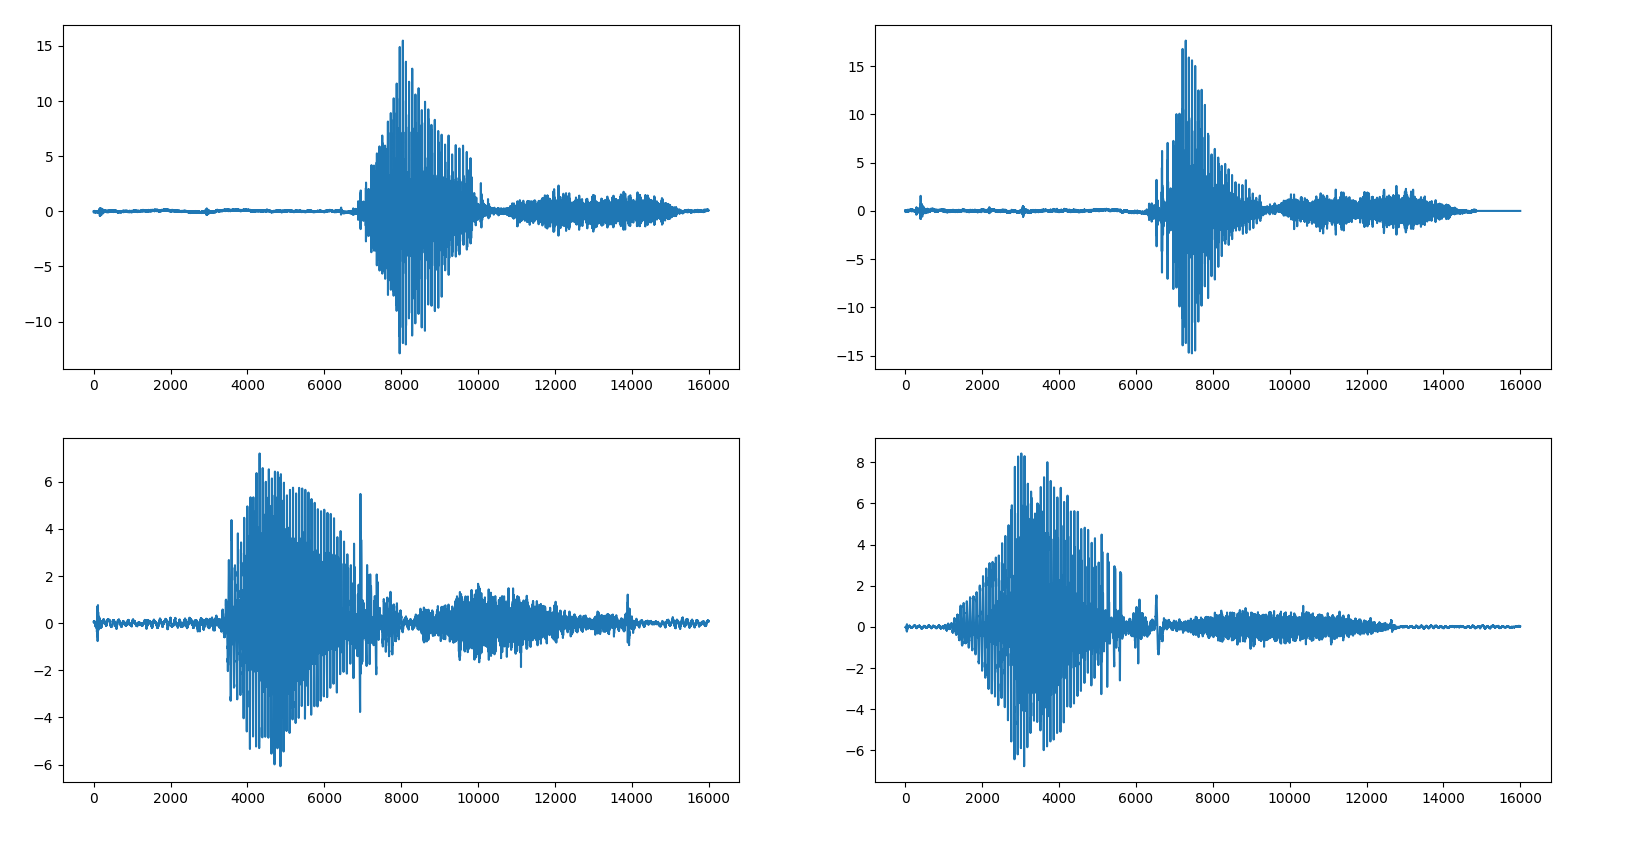
\includegraphics[width=1\textwidth]{chapters/pictures/raw_yes.PNG}
    \caption{a few examples of raw data for the word yes}
    \label{fig:raw_yes}
\end{figure}

But as we can see below, amongst the others examples you will find some that are more or less out of the pattern.


\begin{figure}[!h]
    \centering
    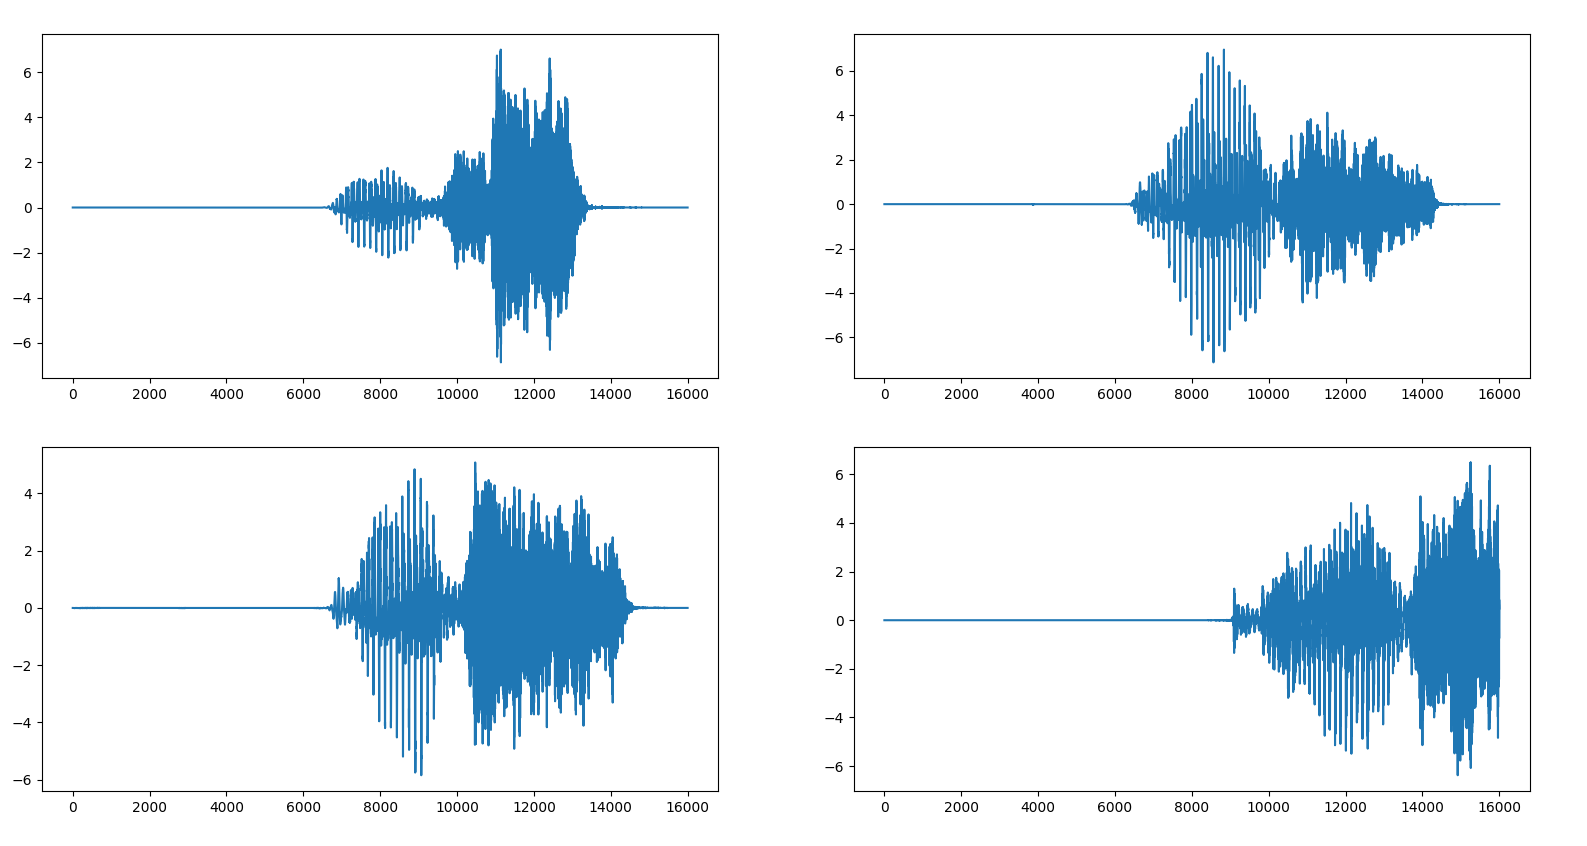
\includegraphics[width=1\textwidth]{chapters/pictures/also_yes.PNG}
    \caption{other examples of yes}
    \label{fig:also_yes}
\end{figure}


\section{Preprocessing data : Mel Frequency Cepstral Coefficients}

The mfcc features are by far the most common way to preprocess audio data \cite{review}. The idea is to represent the power spectrum in a small subset of features over time windows of the signal. The spectrum will be projected on a Mel-scale which is a way to represent the frequencies of a signal closer to how we hear sounds.

\subsection{How do we calculate those coefficients ?}

The method to calculate those coefficients has been taken from here.

\begin{itemize}
    \item The first step is to make time windows of our signal. In our case we take 30ms time windows with a 10 ms step. Which makes us 98 frames.
    \item Then we apply on each frame the discrete fourier transform to obtain an estimate of the power spectrum
    \item Then we compute the Mel-scale filterbanks and apply it the power spectrum
    \item Then we take the log of all filters from the previous step
    \item Finally, apply the discrete cosine transform to those filters
\end{itemize}

This will yields an array of $98 $ x $ n_{filters}$ , $ n_{filters}$ being an arbitrary chosen number between 10 and 40. Usually the number is 13.

\newpage

\subsection{Examples on the word yes}

\begin{figure}[!h]
    \centering
    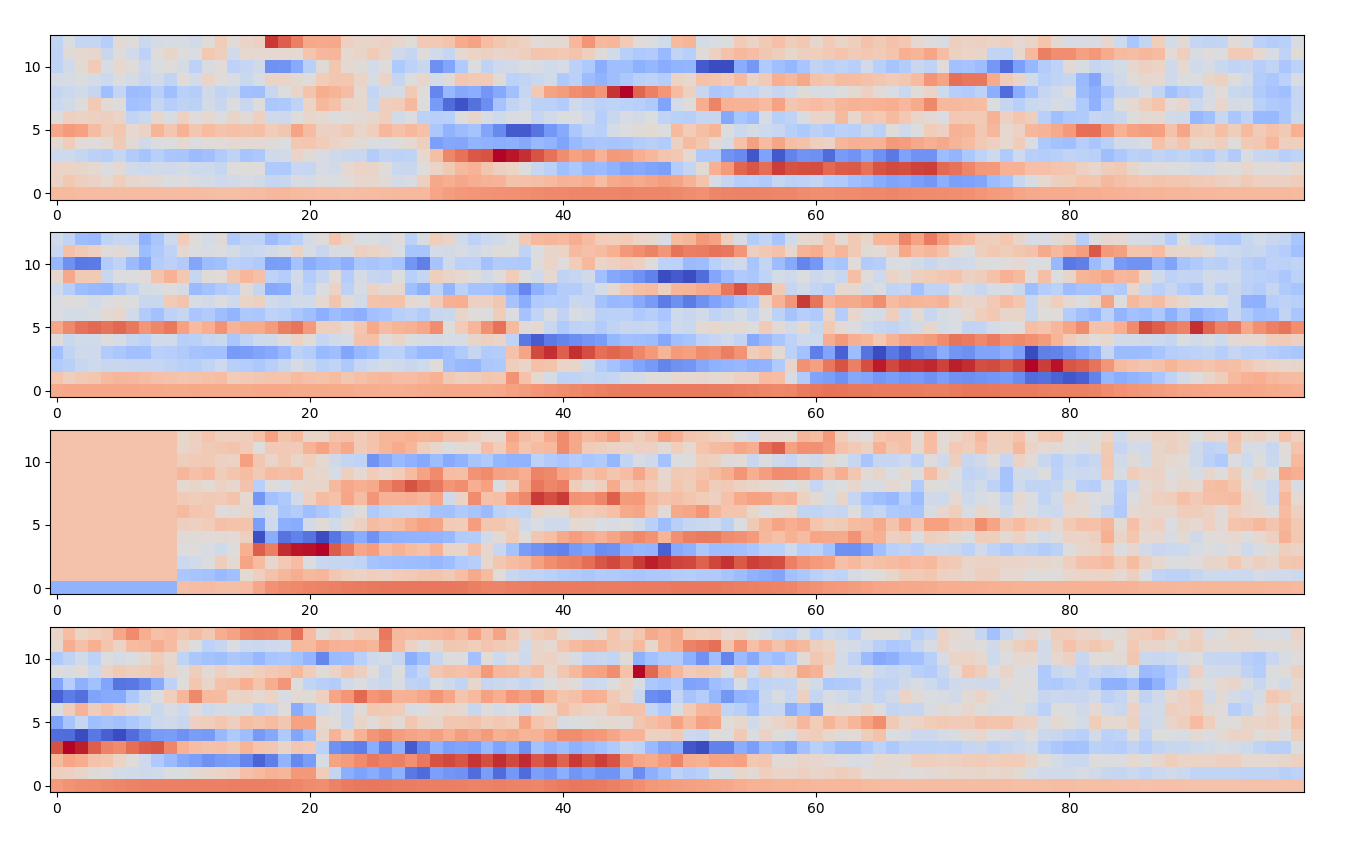
\includegraphics[width=1\textwidth]{chapters/pictures/mfcc_yes.PNG}
    \caption{examples of MFCC features on the word yes}
    \label{fig:mfcc_yes}
\end{figure}

\section{Preprocessing data : Spectral Subband centroids}

To calculate those features, you've to divide the signal into $n_sub$ subbands and take the centroid of each one. The centroid of a subband is the weighted mean of the frequencies in the signal weighted by their magnitude. The number of subbands is arbitrarly chosen (usually 26). You can see the full calculation here \cite{subband}.

\newpage

\begin{figure}[!h]
    \centering
    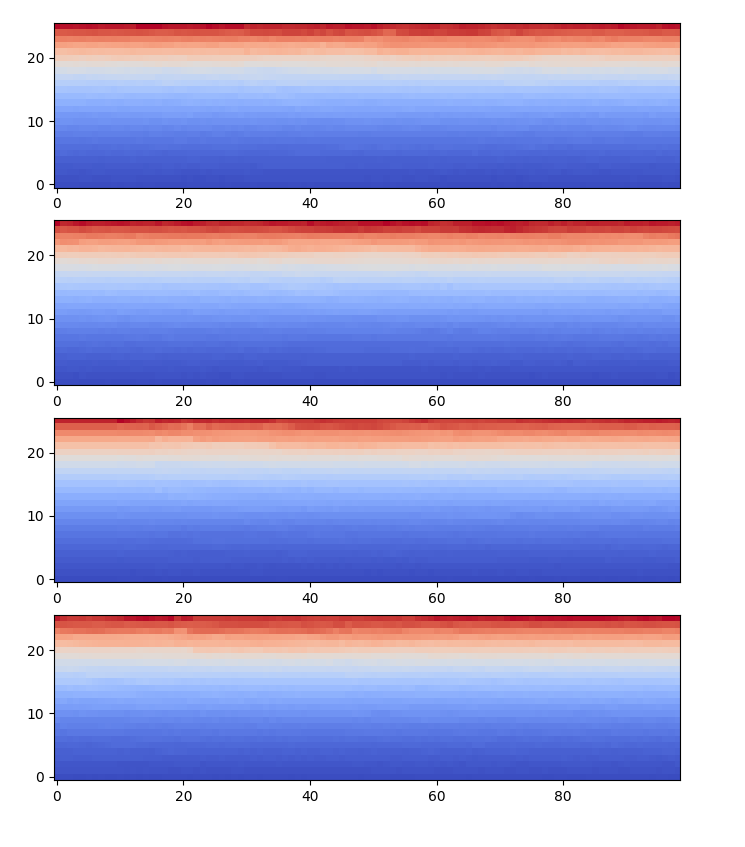
\includegraphics[width=1\textwidth]{chapters/pictures/ssc_yes.PNG}
    \caption{examples of SSC features on the word yes}
    \label{fig:mfcc_yes}
\end{figure}

Those features are extremely different from the mfcc and have been proven to be complementary \cite{subband_comp}. 



\chapter[Related work]{Related work}
\chaptermark{Related work}
There are many types of neural networks and each of them perform differently according to the task. Considering the low vocabulary of our task and the large amount of data, we'll be looking to search for patterns through the identification of templates with neural networks. Therefore, CNN comes immediately to mind. But many works suggests the use of recurrent neural networks. Therefore we'll focus on those two types of networks that seems to be the most promising. Finally, MLPs are usually mentionned but not for their performances, mostly because they are easy to implement and it's always a nice comparison.

\vspace{5mm}

Keyword spotting task are extremely fit to CNNs according to many research CITE GOOGLE. A DNN cannot take advantage of the topology of the signal, however CNNs are extremely good at acoustic modeling which permits to give a good representation of a speech spectrum. The differences of frequencies between each speaker and also the timing differences between each examples are known to be easily handled by CNNs.

\vspace{5mm}

RNNs and especially LSTMs are also fit to this task because of their ability to take into account time sequences through feedback connections. They also benefits from the combination of lstm layers with deep or convolutionnal layers CITEALEX GRAVES. But one of the main problem encountered with RNNs, is that they are slow for many reasons (no parrellelization, slow learning, ...). Therefore the trend is to move away from recurrent structures.






\chapter[Implementation]{Implementation}
\chaptermark{Implementation}
\section{Preprocessing}

The preprocessing part is in the file 'preprocessing.py'. In this file you'll find all functions used to create sub - training, validation and testing lists and the functions that are used to process the data. Since it's better to have a uniform distribution of examples, we decided that we would take a fixed number of example for each label : 2060 examples per label for training, and 206 example per label for the validation. We then create 2266 "silences" for the training and validation. Those silences are created with the background noises given in the dataset.

\subsection{Data}

We use different preprocessing of the data in order to compare or combine them. 

\begin{itemize}
    \item Mel frequency cepstrum coefficients (MFCC)
    \item Spectral subband centroid (SSC)
\end{itemize}

Both mfcc and ssc features are obtained through a python library called python speech features. Then every kind of data is normalized to zero mean and unit variance. The data is then stored into a dictionnary which maps the data (value) to it's kind (key).

\subsection{Labels}

Labels are encoded as a list of length 22 with a one at the index of the right element and zeros otherwise.

\section{Types of neural networks}

To train our networks and implement them we use the tensorflow/keras library. 

\newpage

\subsection{MLP}

\begin{figure}[h!]
    \centering
    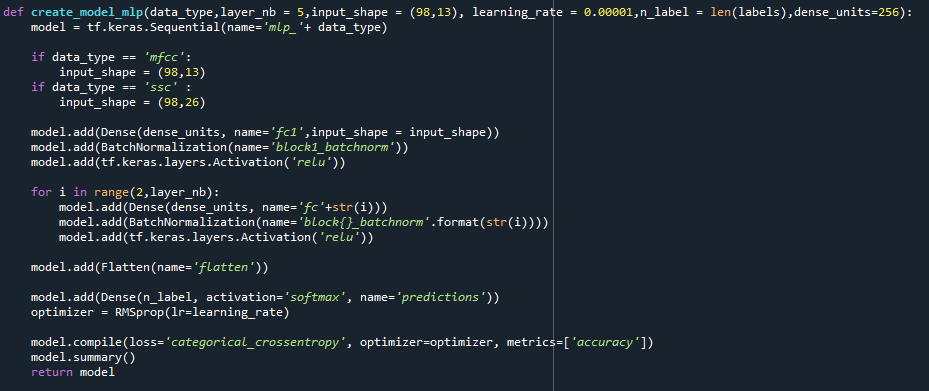
\includegraphics[width=1\textwidth]{chapters/pictures/mlp.PNG}
    \caption{Mlp structure}
    \label{fig:mlp}
\end{figure}

\subsection{CNN}
\subsubsection{Unlimited parameters CNN}

This CNN is around 24M parameters and consists of 5 convolution block with batchnorm and maxpooling. Those 5 convolutions blocks uses 64, 128, 256, 512, 512 filters. Then it uses two denses layers of 4096 neurons with a dropout of 0.5 before each layer to prevent a large overfit.

\begin{figure}[h!]
    \centering
    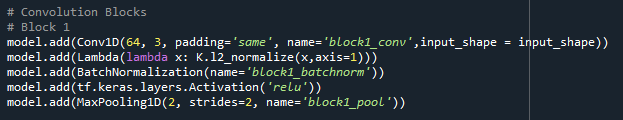
\includegraphics[width=1\textwidth]{chapters/pictures/cnn_block.PNG}
    \caption{Convolutions block}
    \label{fig:cnn_block}
\end{figure}




\begin{figure}[h!]
    \centering
    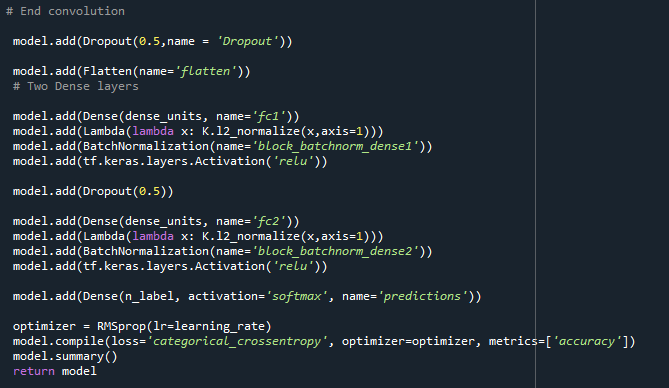
\includegraphics[width=1\textwidth]{chapters/pictures/cnn_end.PNG}
    \caption{Dense layers}
    \label{fig:cnn_end}
\end{figure}

 This makes a really heavy network that we used previously but usually able to learn whatever is asked of him. It's a good starting point. His size being around 200Mo is not extremely pratical for limited embedded devices and therefore we're looking for a smaller network.

\subsubsection{Small CNN < 250k parameters}

The idea behind this network is to try out this trend that stacks convolutions with a lower amount of pooling in a network. To keep it small we uses small numbers of filters and only one dense layer with 200 neurons. No dropout needed because of it's small size, thus we don't waste learned information and we uses the batchnorm layers power to its fullest.

\begin{figure}[h!]
    \centering
    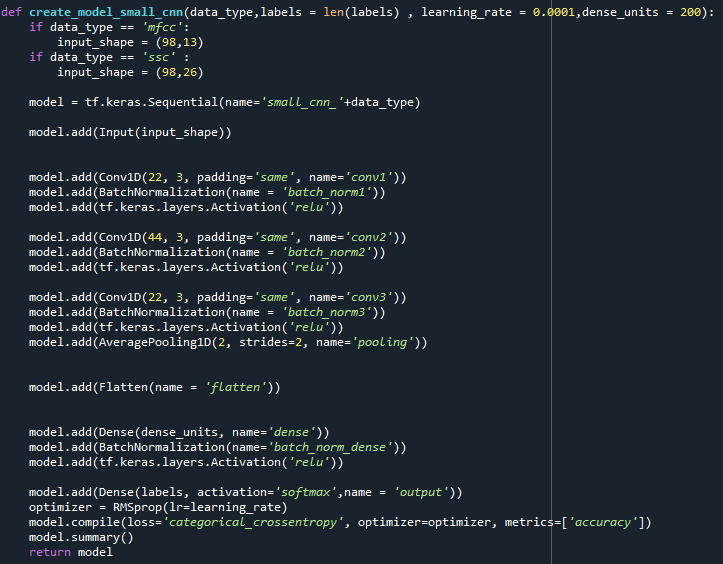
\includegraphics[width=1\textwidth]{chapters/pictures/small_cnn.PNG}
    \caption{Small CNN structure}
    \label{fig:small_cnn}
\end{figure}



\subsection{LSTM}

LSTM can be implemented with a cnn stacked on it therefore the following implementation yields two structure, one is a pure lstm and the other one is a lstm-cnn. The 

\begin{figure}[h!]
    \centering
    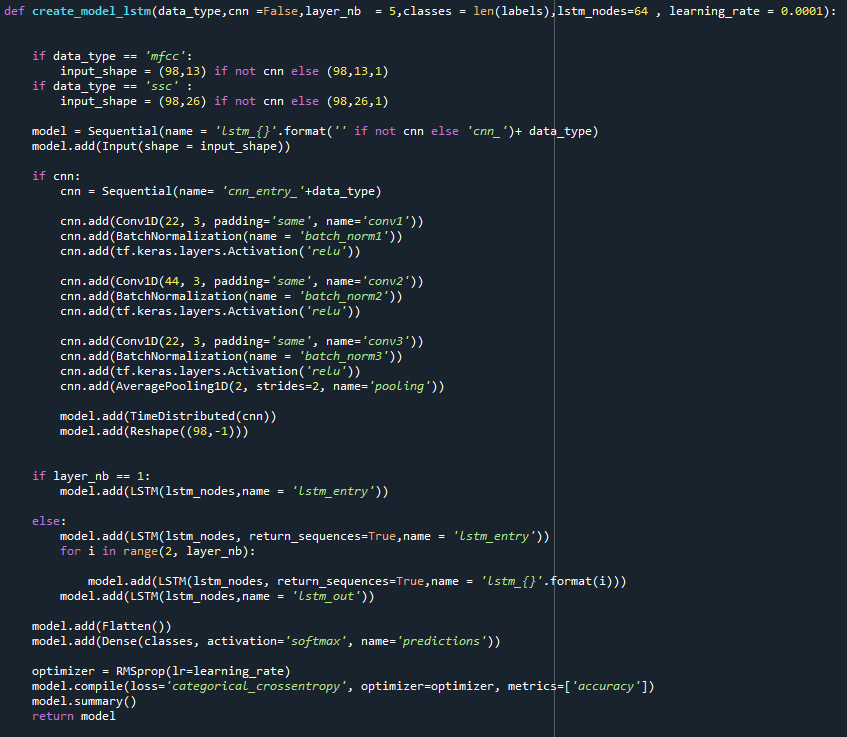
\includegraphics[width=1\textwidth]{chapters/pictures/lstm.PNG}
    \caption{Lstm structure}
    \label{fig:lstm}
\end{figure}




\chapter[Results]{Results}
\chaptermark{Results}

\begin{table}[h!]
    \centering
    \begin{tabular}{|c|c|}
        
        
        \hline
        Model & Accuracy \%  \\
        \hline
        DenseNet-121 best & 85.52 \\
        \hline
        ConvNet & 85.4 \\
        \hline
        Attention RNN best & 94.5 \\
        \hline
        Kaggle winner & 91.06\\
        \hline        
    \end{tabular}
    \caption{Public Accuracy on the Google Data dataset v1 20words \cite{ATTRNN}}
    \label{tab:general}
\end{table}

Those results have been achieve on differents subsets of the testing list that we have. The testing list that i have is the combination of the public test set for the kaggle challenge and the private test set. Therefore the accuracy achieved by the kaggle winner is only on the private test set. The others have been tested on the original test set which is the public and private test set of the kaggle challenge. But the label "silence" hasn't been added to the learning task. We have one more label than them.


\section{Test definition and metrics}


To do the test we use the original testing list provided by the author of the data set which is around 6000 files. We add also 200 silences that are obtained with various chunks of the background files, which are'nt taken into account in the tests sets of the figure \ref{tab:general}.

\vspace{5mm}
In order to judge our networks, we use 4 metrics.

\vspace{5mm}

Let $t_p, f_p, t_n, f_n$ be the number of true positives, false positives, true negatives and false negatives. We define our metrics the following way :

\begin{itemize}
    \item Precision : $P = \frac{t_p}{t_p + f_p}$
    \item Recall : $R = \frac{t_p}{t_p + f_n}$
    \item False positive rate : $Fpr = \frac{f_p}{t_p + f_p + t_n + f_n}$
    \item Accuracy : $A = \frac{t_p + t_n}{t_p + f_p + t_n + f_n}$
\end{itemize}

\section{General results}

\begin{table}[h!]
    \centering
    \begin{tabular}{|c|c|c | c |c |c|}
        
        
        \hline
         & $MLP$ & $CNN_{250k}$ & $CNN$ & $LSTM_{cnn}$ & $LSTM$  \\
        \hline
        Success rate MFCC & 97.58 & 98.54 & 99.33 & 97.57 & 97.37\\
        \hline
        Success rate SSC & 96.19 & 92.75 & 97.17 & 96.33 & 28.20\\
        \hline
    \end{tabular}
    \caption{Success rates for all models and preprocessing}
    \label{tab:genera_modell}
\end{table}

As expected the most complex network as the best accuracy in both preprocessing. Also MFCC preprocessing wins everytime and SSC preprocessing seems to not work at all on pure lstms layers. 



\section{MLP}





As we can see in the table \ref{fig:table_mlp} and in the heatmap below, that most of the mistakes made by the MFCC preprocessing are coming from "down", "three", "eight", "nine" and "off". "down" and "three" are likely to be confused with "dog" and "tree" in the unknown set. "eight" is quite often confused with four. "nine" and "off" also with the unknown set but with no clear antagonist.

\begin{figure}[h!]

    \centering
    \subfloat[\centering MFCC preprocessing]{{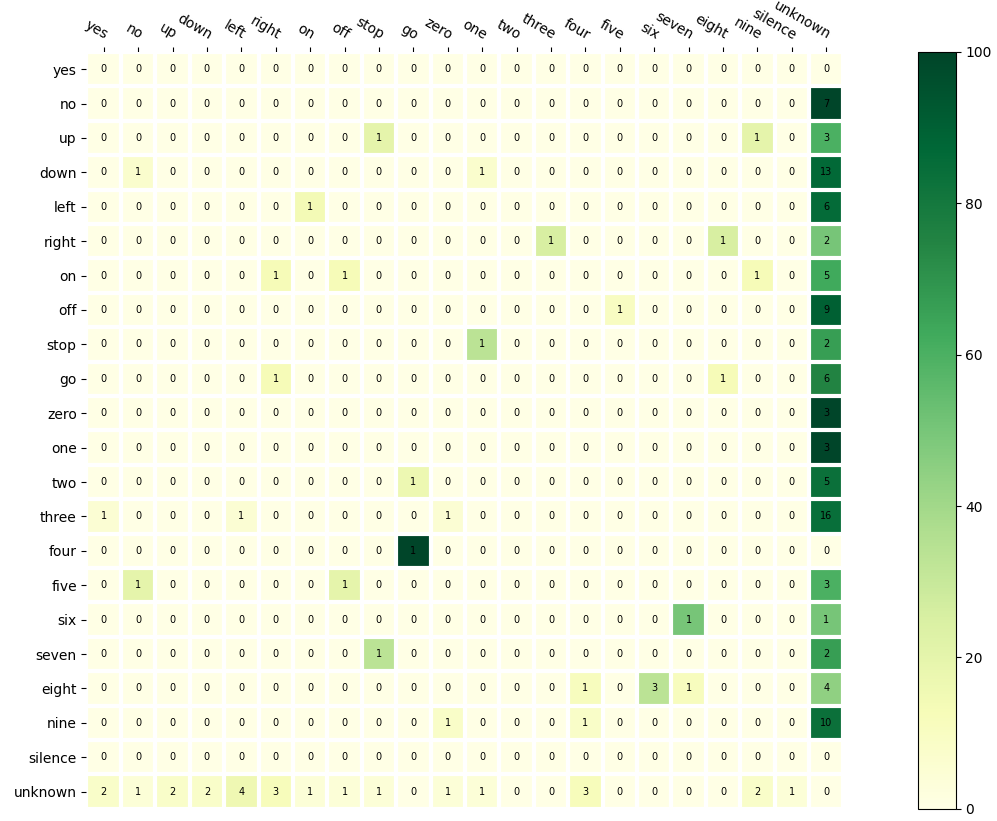
\includegraphics[width=6cm]{chapters/pictures/mlp_mfcc_heatmap.PNG} }}
    \qquad
    \subfloat[\centering SSC preprocessing]{{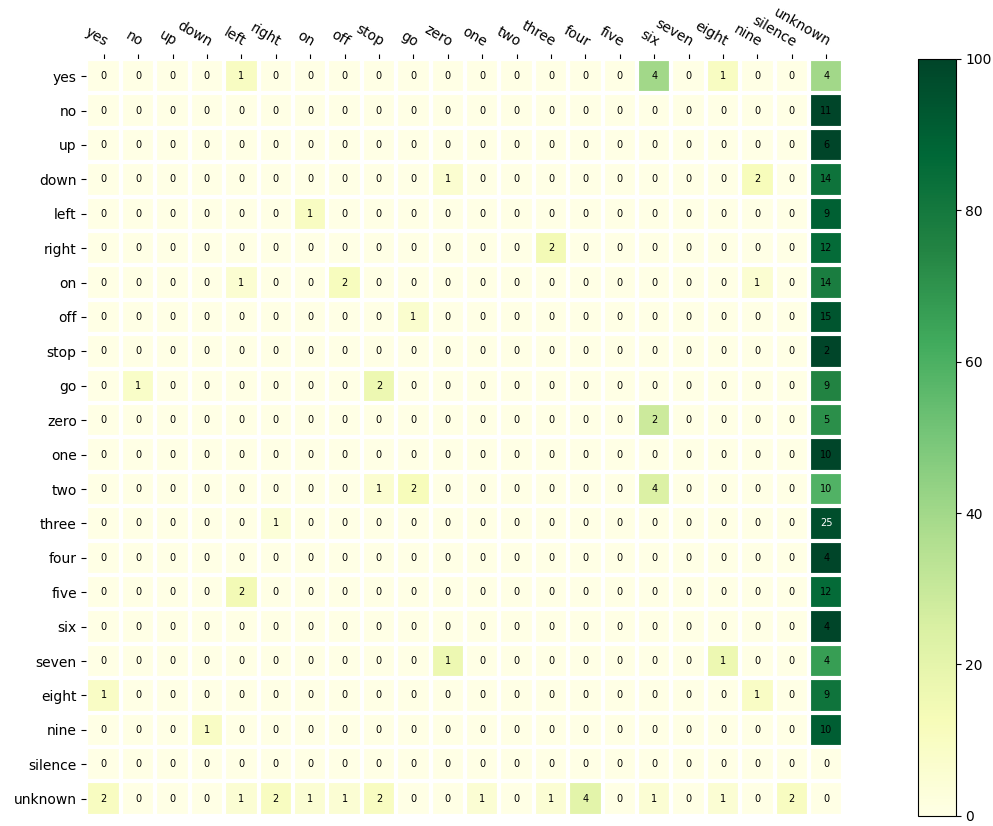
\includegraphics[width=6cm]{chapters/pictures/mlp_ssc_heatmap.PNG} }}
    \caption{Confusion matrix for MLPs with different preprocessing}
    \label{fig:confusion_mlp}

\end{figure}

What we can see is that in general the SSC preprocessing has a classify a lot of out of the ordinary examples in the unknown label. So does the MFCC but with more success.

\newpage

\section{CNN}




From this table \ref{fig:table_cnn} we can see that most of the labels are almost always recognized perfectly with the mfcc preprocessing, but again we see some problems for "three" and "eight". It's even clearer when we look at the heatmap. There is a much higher confusion for "three" than for the others.



\begin{figure}[h!]

    \centering
    \subfloat[\centering MFCC preprocessing]{{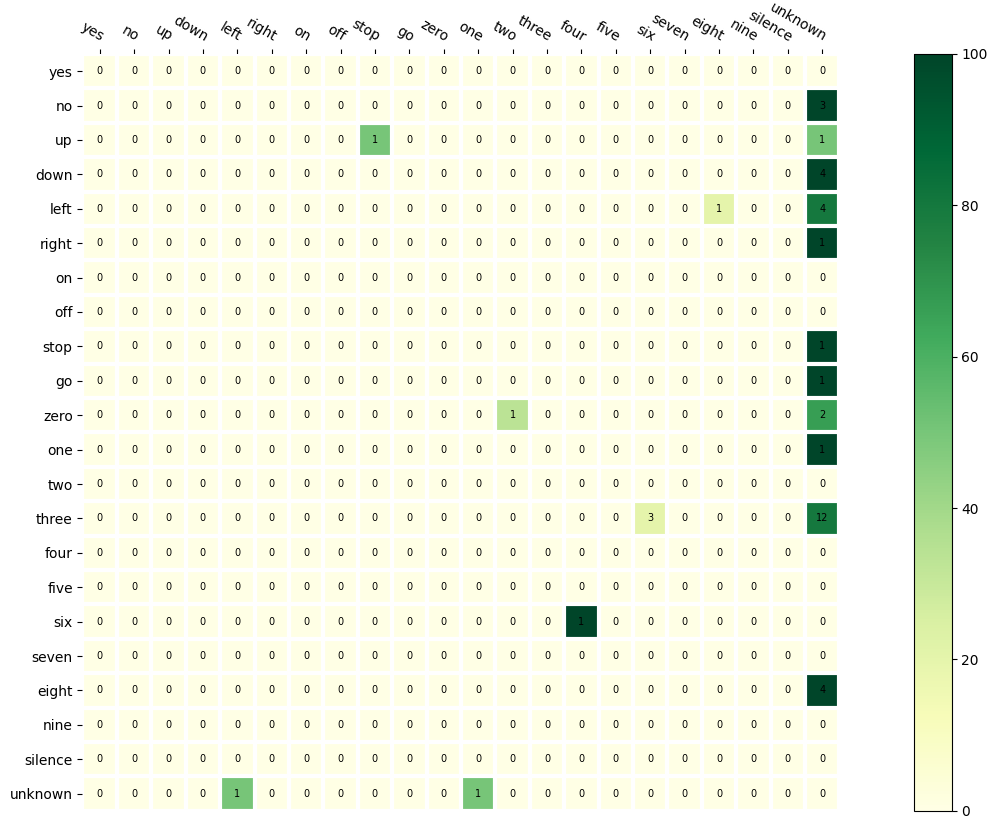
\includegraphics[width=6cm]{chapters/pictures/heatmap_cnn.PNG} }}
    \qquad
    \subfloat[\centering SSC preprocessing]{{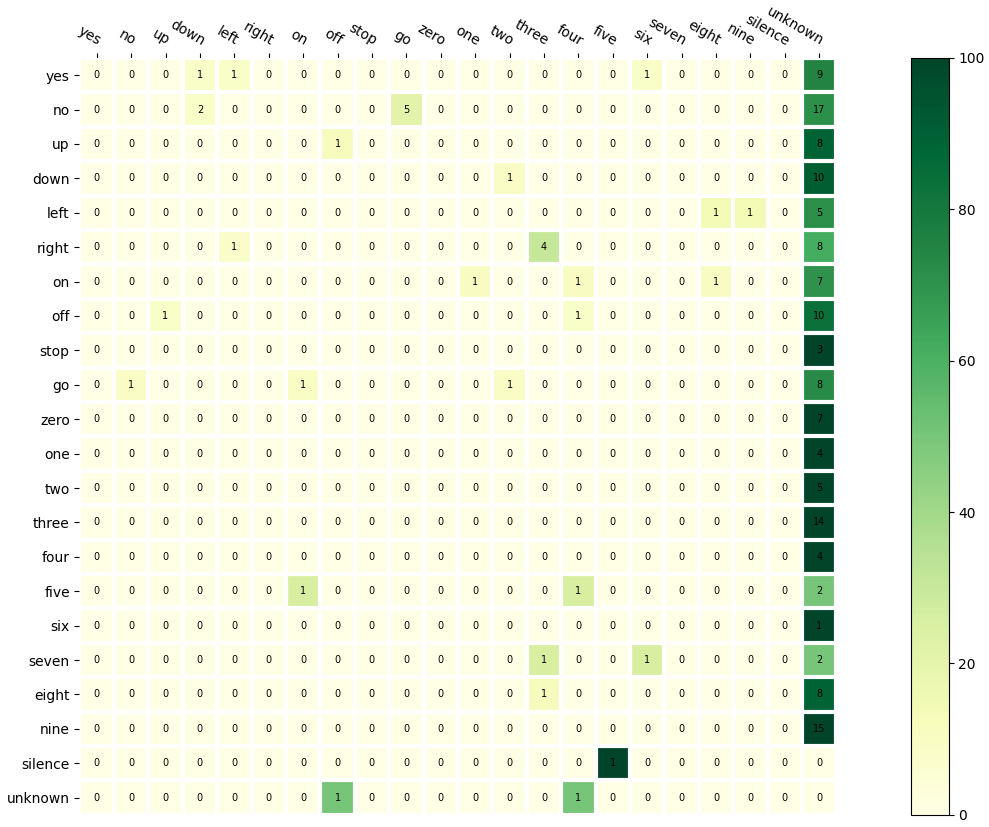
\includegraphics[width=6cm]{chapters/pictures/heatmap_cnn_ssc.PNG} }}
    \caption{Confusion matrix for CNNs with different preprocessing}
    \label{fig:confusion_cnn}

\end{figure}


\newpage



Results for the smaller models are in this table \ref{fig:table_small} .With a smaller model, we can see that "three" is still a problem, so is "nine" but we have a new problematic label emerging which is "no"

\begin{figure}[h!]

    \centering
    \subfloat[\centering MFCC preprocessing]{{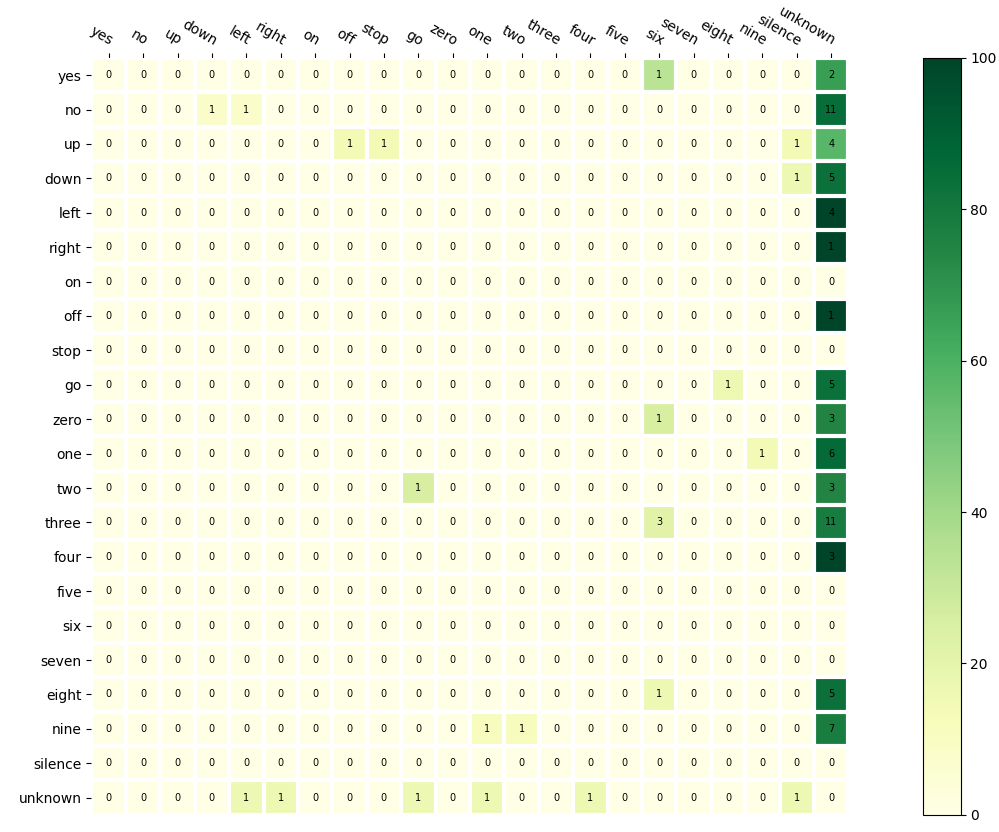
\includegraphics[width=6cm]{chapters/pictures/small_matrixmfcc.PNG} }}
    \qquad
    \subfloat[\centering SSC preprocessing]{{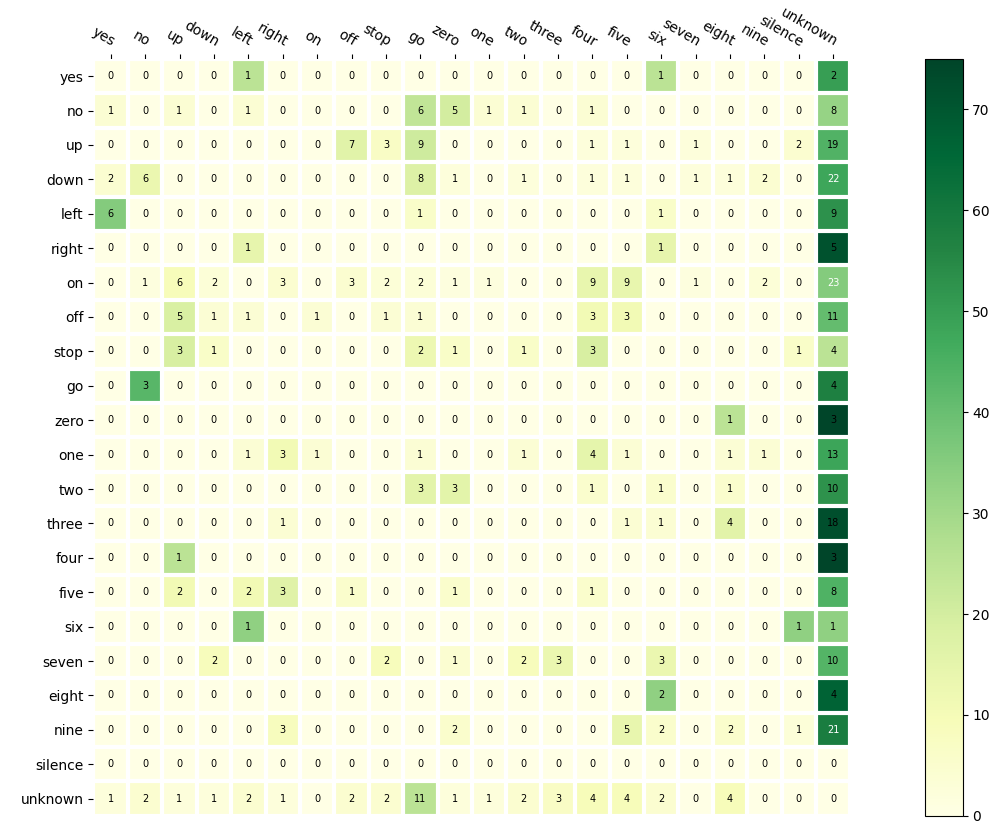
\includegraphics[width=6cm]{chapters/pictures/small_matrix_ssc.PNG} }}
    \caption{Confusion matrix for small CNNs with different preprocessing}
    \label{fig:confusion_small}

\end{figure}


\section{LSTM}




In lstm we can see that the ssc preprocessing is not giving any results. Looks like the structure is not able to learn anything. We didn't plot the heatmap for the ssc preprocessing because there was no point. It's just not accurate at all.

\begin{figure}[h!]
    \centering
    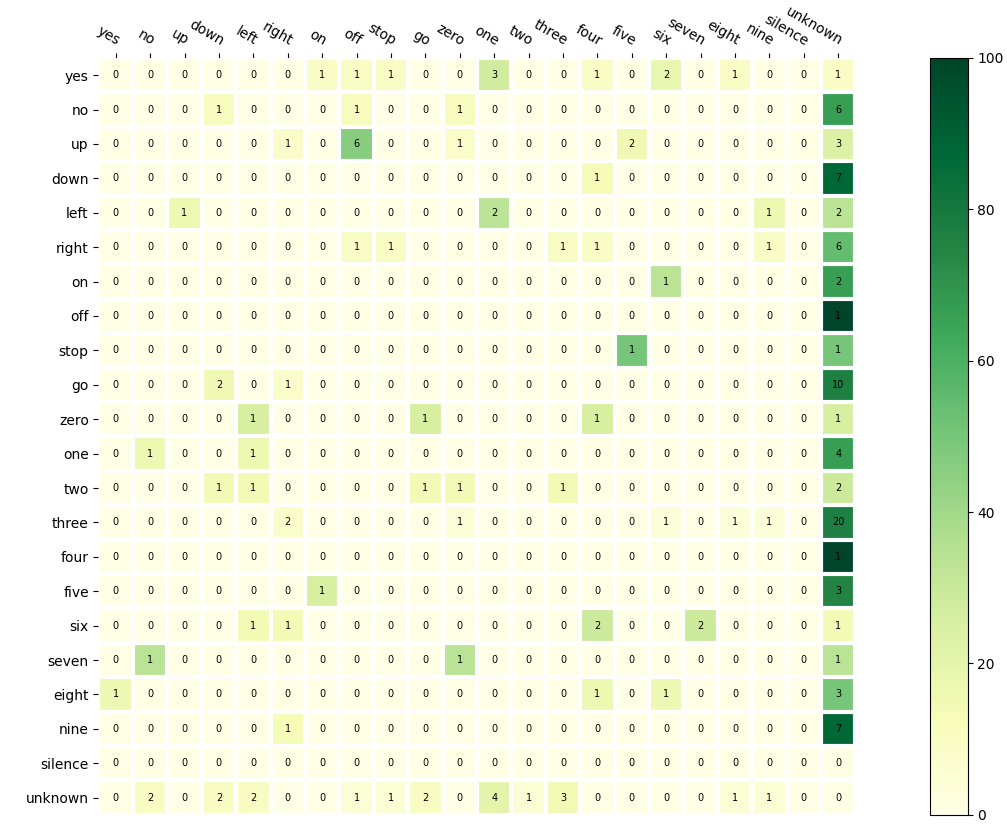
\includegraphics[width=0.5\textwidth]{chapters/pictures/lstm_matrix_mfcc.PNG}
    \caption{Confusions matrix for LSTM and MFCC}
    \label{fig:matrix_lstm_mfcc}
\end{figure}

\newpage

What we can see on the other hand is that the confusions looks like more distributed over the labels. Where usually the only confusions were giving a false unknown label, we have less false positives for the unknown label and more conufusion between regular labels. Still we have a few labels with really inaccurate results like "three".



\begin{figure}[h!]

    \centering
    \subfloat[\centering MFCC preprocessing]{{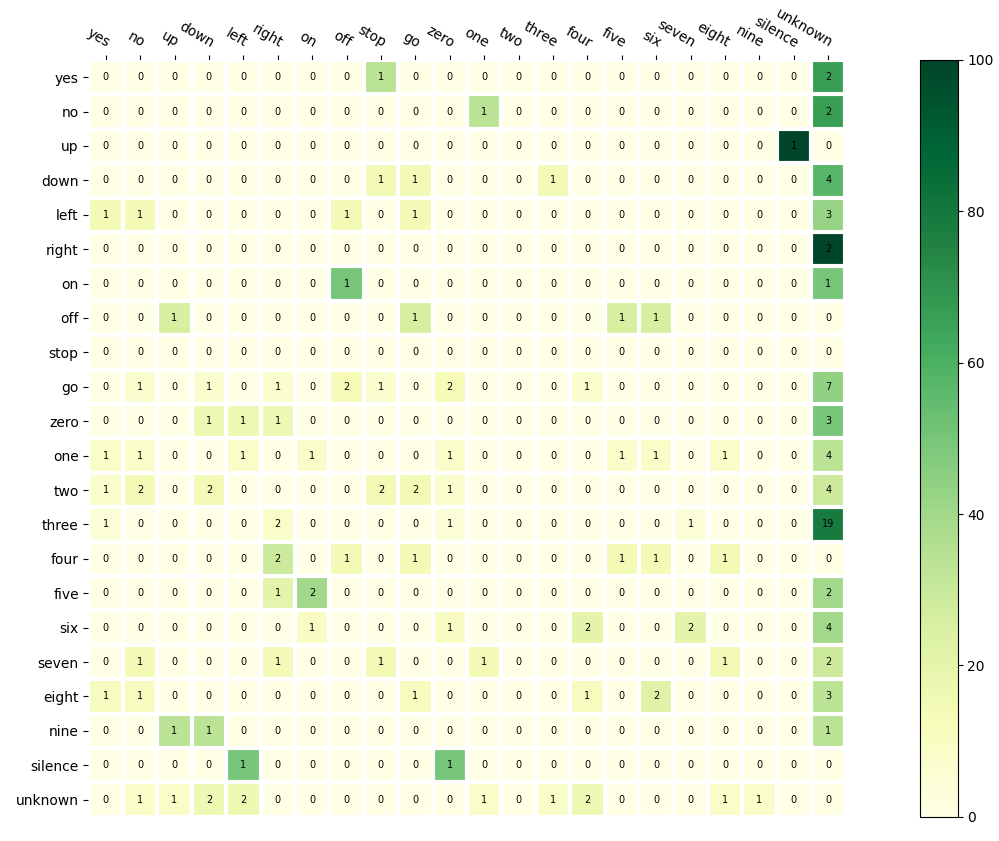
\includegraphics[width=6cm]{chapters/pictures/lstm_cnn_heatmap.PNG} }}
    \qquad
    \subfloat[\centering SSC preprocessing]{{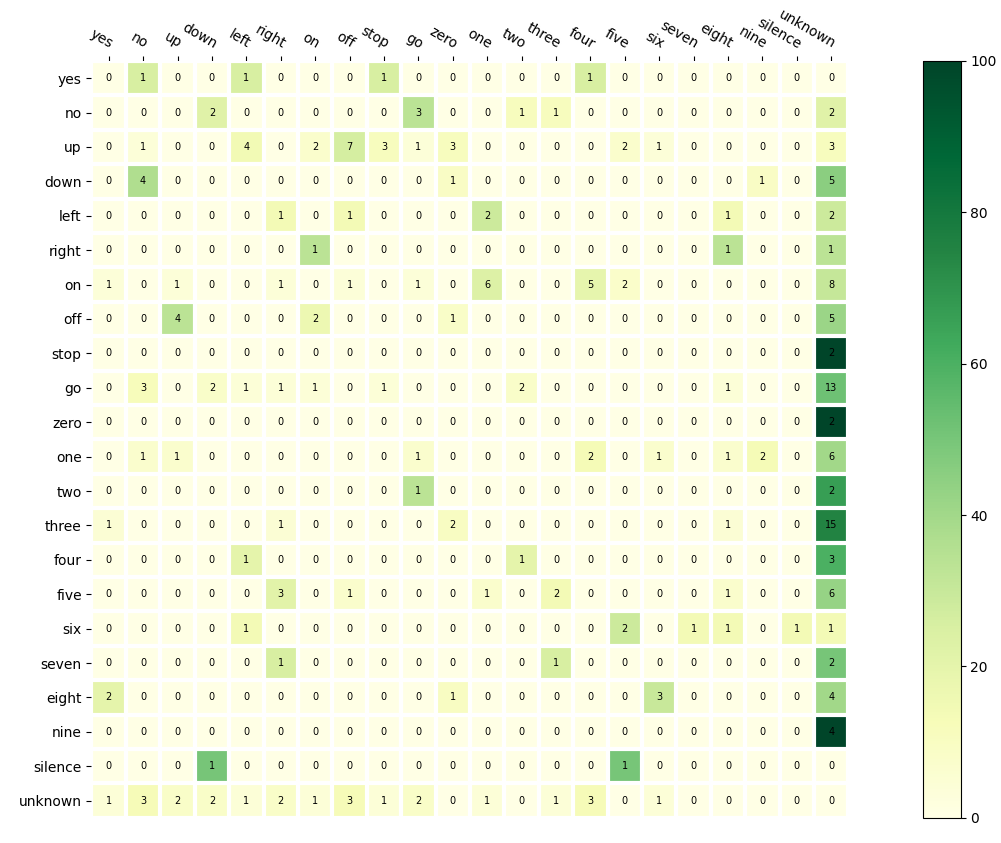
\includegraphics[width=6cm]{chapters/pictures/lstm_cnn_heatmap_ssc.PNG} }}
    \caption{Confusion matrix for LSTM CNN with different preprocessing}
    \label{fig:confusion_lstm_cnn}

\end{figure}

Same results than with the pure lstm in term of distributions of inaccuracies. But we solved the issue of the ssc preprocessing by adding a convolutionnal layer before hand.



\section{Conclusion}

To conclude, we have a few problematic labels, mostly "three". It makes sense since "tree" is present as an unknown word. The differenciation between those two words in the english language is mostly done with the context of the phrase. Here, there is no context. We think that a human would make a significant amount of mistakes if he tried to do the same. We can also see that CNNs and MLPs are classifying more often a word as an unkwown word where lstm are making more mistakes by classifying one known label with another. It would mean that for the CNNs and MLPs, the "templates" created when the model learns are more strict. Therefore when one example is out of the ordinary, it's is classified as an unknown word. While for LSTMs, those templates are more flexible, thus rejecting less words but making more mistakes. We believe that if we were to use one of this network in practice, we would choose a CNN. Because it's better to think that something is unknown than thinking something is true while it's not.


\chapter[Conclusion]{Conclusion}
In this work we tried different structures and preprocessing to achieve the classification of some one word commands. We saw that for our models a convolution is needed to achieve good performances. The best model is the most complex CNN but closely followed but the LSTM with a convolution and a smaller CNN, which are both networks with under 250k parameters. The MFCC preprocessing is clearly the winner as expected. We achieve a much better accuracy than the one that we've been able to find but we have an additional label that has 100\% accuracy. Even without it though, the accuracy is better. During this work we've been through an idea called ensemble machine learning and even if we didn't demonstrated here we found some interesting results during live tests. Ensemble machine learning make more robust to input twists predictions if the networks that are combined do not learn the same thing. But since the idea here was to keep the footprint low, we decided not to use it.
\printbibliography
%%%% Bibliography before appendices
%%%% After the initial round, you need to fix it by hand depending on where you generate your .bib file from
%%%% Mendeley often messes with italics and accents for instance


% Appendices
\begin{appendices}
\begin{figure}[h!]
    \centering
    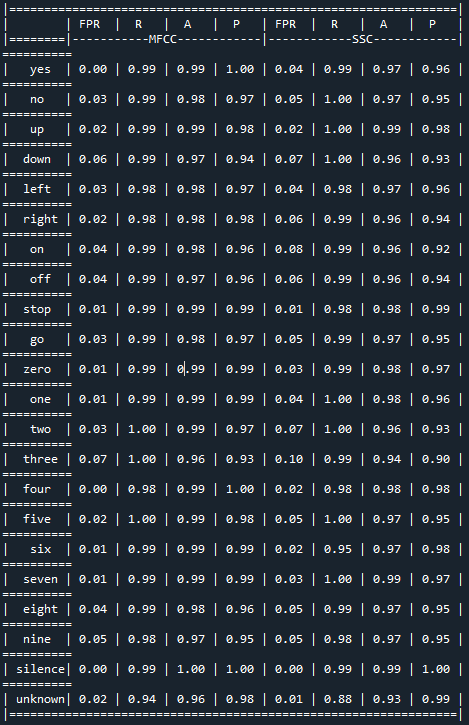
\includegraphics[width=1\textwidth]{chapters/pictures/table_mlp.PNG}
    \caption{Metrics for each label with MLP}
    \label{fig:table_mlp}
\end{figure}
\newpage
\begin{figure}[h!]
    \centering
    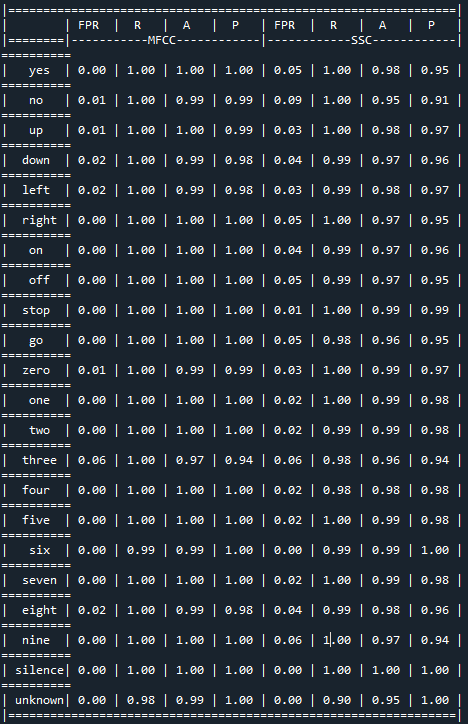
\includegraphics[width=1\textwidth]{chapters/pictures/table_cnn.PNG}
    \caption{Metrics for each label with CNN}
    \label{fig:table_cnn}
\end{figure}
\newpage
\begin{figure}[h!]
    \centering
    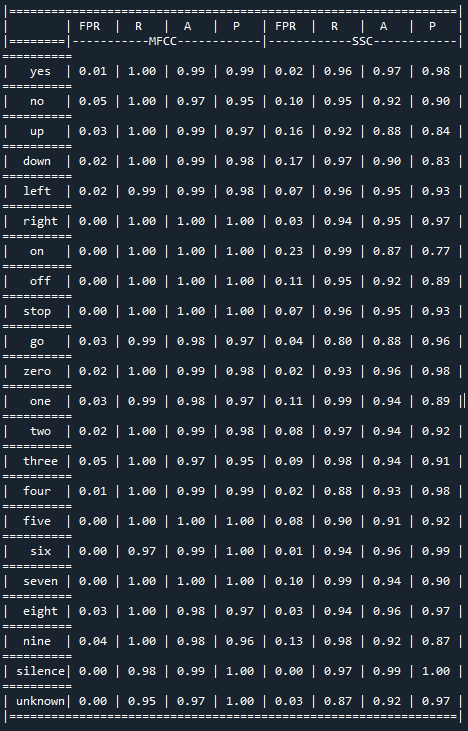
\includegraphics[width=1\textwidth]{chapters/pictures/table_small.PNG}
    \caption{Metrics for each label with a small CNN}
    \label{fig:table_small}
\end{figure}
\newpage
\begin{figure}[h!]
    \centering
    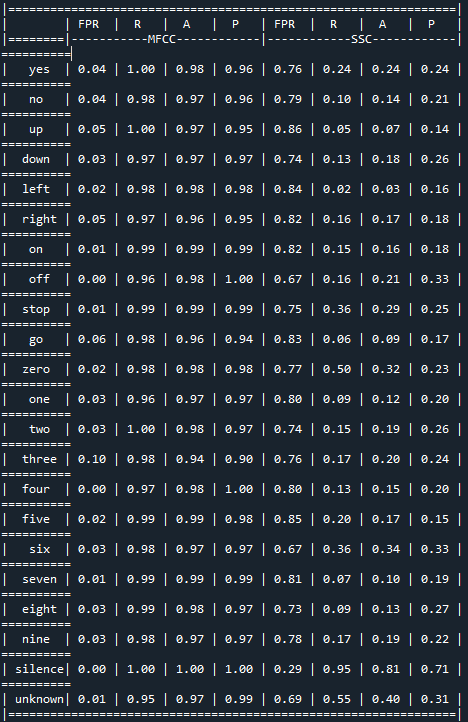
\includegraphics[width=1\textwidth]{chapters/pictures/lstm_table.PNG}
    \caption{Metrics for LSTM}
    \label{fig:table_lstm}
\end{figure}
\newpage
\begin{figure}[h!]
    \centering
    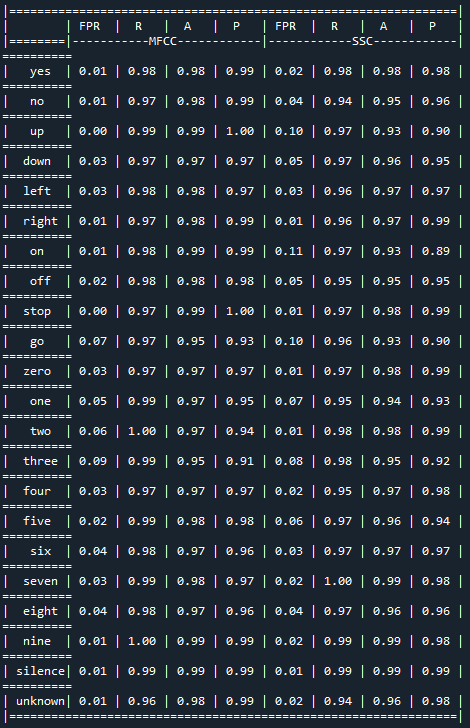
\includegraphics[width=1\textwidth]{chapters/pictures/lstm_cnn_table.PNG}
    \caption{Metrics for LSTM + CNN}
    \label{fig:table_lstm_cnn}
\end{figure}
\newpage
\end{appendices}

\end{document}